\documentclass[10pt,twocolumn,letterpaper]{article}

\usepackage{cvpr}
\usepackage{times}
\usepackage{epsfig}
\usepackage{graphicx}
\usepackage{float}
\usepackage{amsmath}
\usepackage{amssymb}
\usepackage{enumitem}

\usepackage[top=0.7in, bottom=0.7in, left=0.7in, right=0.7in]{geometry} % Adjust margins here

\usepackage[breaklinks=true,bookmarks=false]{hyperref}

\cvprfinalcopy

\def\httilde{\mbox{\tt\raisebox{-.5ex}{\symbol{126}}}}

\setcounter{page}{1}
\begin{document}

\title{\begin{center}
    \vspace{-1.75cm}
    DeepDetect : Detect Fake and AI-generated Images
\end{center}
End-Semester Project Report}

\author{Himang Chandra Garg \qquad Dasari Sai Harsh \qquad Nishil Agarwal \qquad Piyush Narula\\
Indraprastha Institute of Information Technology, Delhi\\
{\tt\small \{himang22214, dasari22144, nishil22334, piyush22354\}@iiitd.ac.in}
}

\maketitle

\pagestyle{empty}

%-------------------------------------------------------------------------

\begin{abstract}

Our project seeks to address the critical issue of detecting deepfake images and AI-generated content, which have become increasingly sophisticated and challenging to distinguish from real media. 
The objective is to enhance the ability to discern genuine content from fabricated images, thereby reducing the potential for misinformation.
We have explored various machine learning techniques, including Support Vector Machines (SVM), Random Forests, and Convolutional Neural Networks (CNNs), to classify images as real or fake and compared the effectiveness of traditional ML models and CNNs.
Github link : \url{https://github.com/himangg/Machine-Learning-Project}
\end{abstract}

\vspace{-5pt}
\section{Introduction}
\subsection{Problem Statement and its Significance}

The recent rise in AI content, particularly deepfake images and videos, has raised serious concerns about the integrity of information online. 
This synthetic media is often indistinguishable from real content, hence making it very difficult for an average person to tell the truth—an aspect with large implications in public trust, privacy, and security.
Our project aims to develop a robust system capable of detecting AI-generated images, thereby helping to combat the spread of misinformation and fake content.

%------------------------------------------------------------------------
\section{Literature Survey}
Detecting fake images with machine learning is a difficult and growing research field because image editing tools are becoming more accessible and user-friendly. Recent studies have focused on creating automated systems utilizing machine-learning methods in order to identify counterfeit images. This review of literature outlines the latest research in this area and addresses the difficulties and future paths ahead using the following 2 papers.
\subsection{\href{https://ijrpr.com/uploads/V4ISSUE4/IJRPR11629.pdf}{Detecting Fake Images Using Machine Learning}}
The paper "Detecting Fake Images Using Machine Learning" by Mr. Akash K, Miss. Ahalya K, Mr. Dhinesh N, Miss. Diya Shereef delves into strategies for detecting manipulated images using both traditional image processing and machine learning approaches. The writers suggest a combination model that uses CNNs to extract features like color patterns, texture, and statistical characteristics from images. Next, these characteristics are inputted into a classifier that differentiates between authentic and altered images. The suggested model attains high accuracy and can be utilized in social media content moderation, news verification, and forensic investigations.

\subsection{\href{https://www.researchgate.net/publication/375952278_Deep_Learning_for_Image_Authentication_A_Comparative_Study_on_Real_and_AI-Generated_Image_Classification}{Deep Learning for Image Authentication: A Comparative Study on Real and AI-Generated Image Classification}}
The effectiveness of deep learning models in differentiating real images from AI-generated ones is investigated in the paper "Deep Learning for Image Authentication: A Comparative Study on Real and AI-Generated Image Classification" by Gaye Ediboglu Bartos and Serel Akyol. The research is centered around two models: Residual Networks (ResNet) and Variational Autoencoders (VAEs). ResNet, renowned for its strong feature extraction abilities, reached an impressive 94\% accuracy in distinguishing between real and synthetic images in the CIFAKE dataset, comprising 60,000 real and 60,000 AI-generated images. On the other hand, VAEs, taking an anomaly detection stance, had a lower accuracy of 71\% because of their generative nature and less discriminative architecture. The paper highlights how crucial it is to tune hyperparameters, such as batch sizes and epochs, in order to improve model performance.

\section{Dataset: Exploratory Data Analysis}
We have used \href{https://www.kaggle.com/datasets/manjilkarki/deepfake-and-real-images}{this} dataset.This dataset contains manipulated images and real images. The manipulated images are the faces which are created by various means. Each image is a 256 X 256 jpg image of human face either real or fake
By using bar graphs, scatter plots, and violin plots, we analyze the similarities in image size, color distribution, and saturation variances between authentic and AI-produced images. 
This examination assists in recognizing possible disparities in class, variations in features, and discrepancies.
\subsection{Visualization of Dataset}
\begin{itemize}
    \item \textbf{Class Imbalance Graphs:} In order to avoid overfitting, we analyzed the amount of images per category in both the training and validation sets. If there were a large imbalance in the number of images in a class, we would have conducted undersampling to achieve a more equal distribution in the dataset. 
    We found no significant class imbalance.
    \begin{figure}[H]
    \centering
    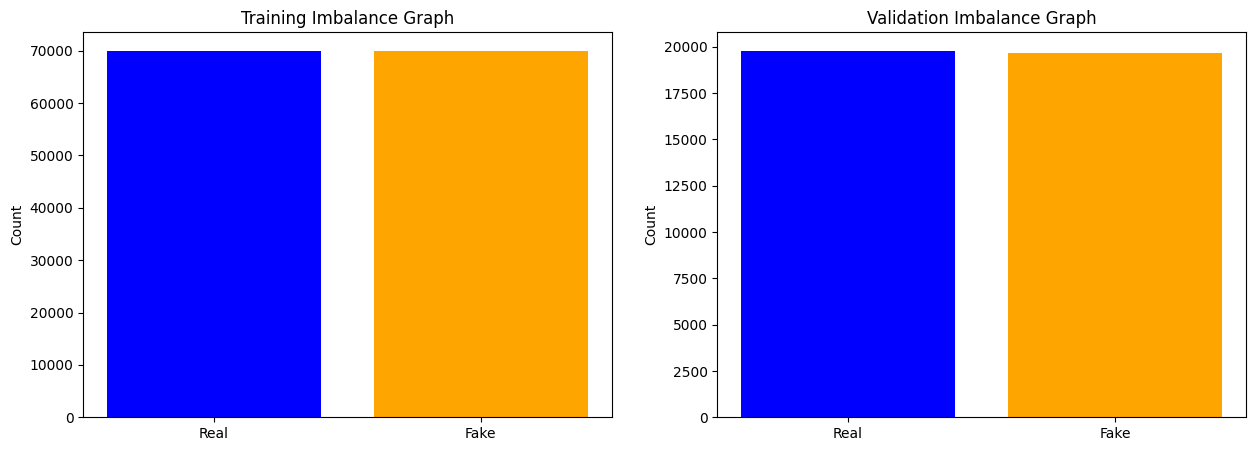
\includegraphics[scale=0.2]{2.png}
    \end{figure}
    \item \textbf{Scatter plot of face dimensions:} Faces were extracted from images for deepfake detection. A width vs height scatterplot was created but did not show a difference between real and fake image dimensions, suggesting it may not help distinguish them.
    \begin{figure}[H]
    \centering
    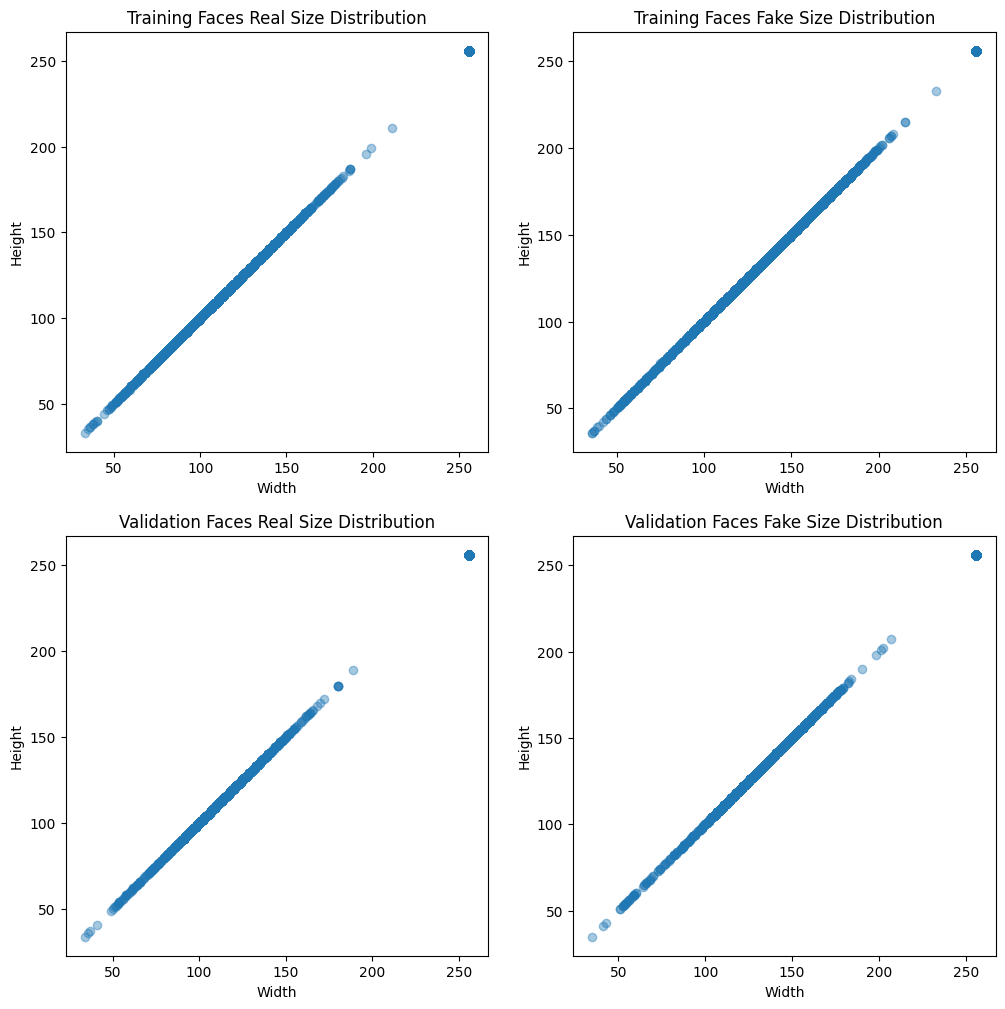
\includegraphics[scale=0.2]{3.png}
    \end{figure}
    
    \item \textbf{Mean Real and Fake Face images:} We created a visual representation of the average face extracted from both the real and fake image datasets in order to compare the mean face images of each type. We noticed distinct discrepancies since they did not resemble each other.
    \begin{figure}[H]
    \centering
    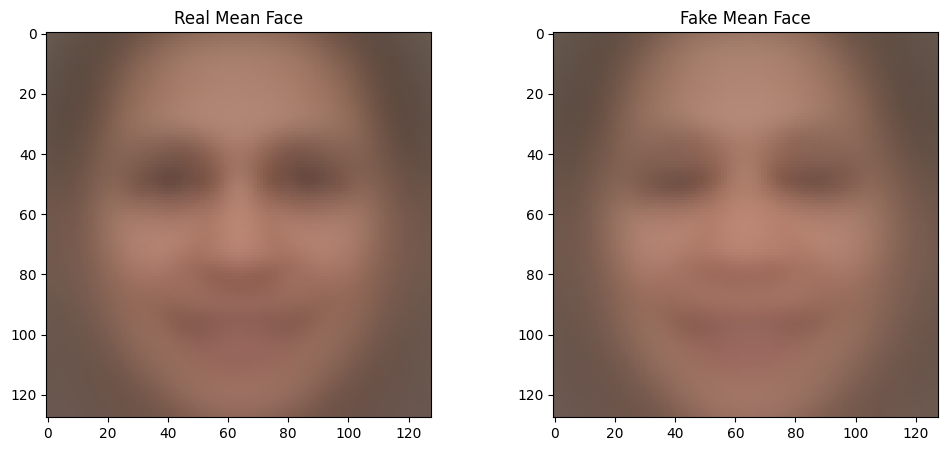
\includegraphics[scale=0.2]{4.png}
    \end{figure}

    \item \textbf{RGB Intensity Violin Plots:} RGB intensities were extracted using colour histograms from real and fake face datasets. Average frequency of intensity pixels in both datasets was calculated. Violin plots were created to compare RGB differences between real and fake images. Some differences were observed but they do not seem that significant.
    \begin{figure}[H]
    \centering
    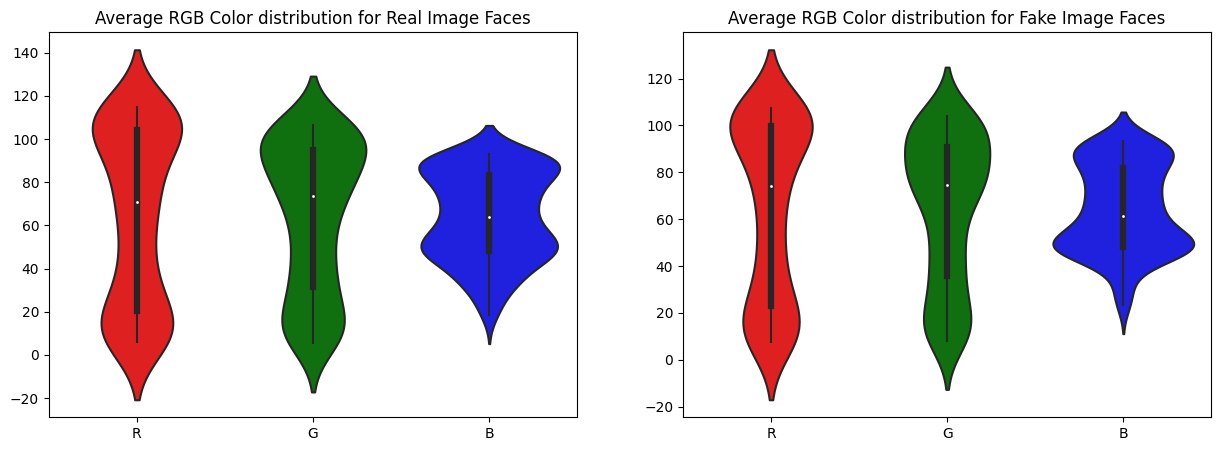
\includegraphics[scale=0.2]{5.png}
    \end{figure}

    \item \textbf{Box plot for Colour Saturation:} We extracted colour saturation from real and fake face datasets. We generated box plots on basis of the saturation data. We observed no significant differences.
    \begin{figure}[H]
    \centering
    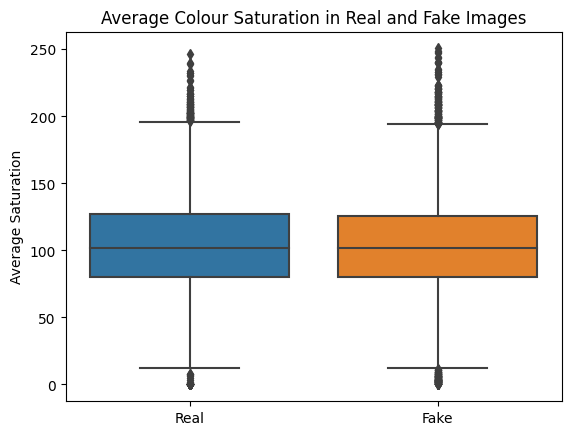
\includegraphics[scale=0.3]{6.png}
    \end{figure}

\end{itemize}


\section{Methodology: Preprocessing and Model}
\subsection{Classical Machine Learning}

\subsubsection{Pre-processing and Data Augmentation}

Pre-processing and data augmentation improve model performance by standardizing data and expanding dataset.
\subsubsection{Data Augmentation Techniques}

\begin{itemize}
    \item Spatial Transformations
    
    \item Image Quality Transformations through noise 
    
    \item Color Transformations
    
    \item Mild Distortions
\end{itemize}

\subsubsection{Methodology}

\begin{figure}[H]
    \centering
    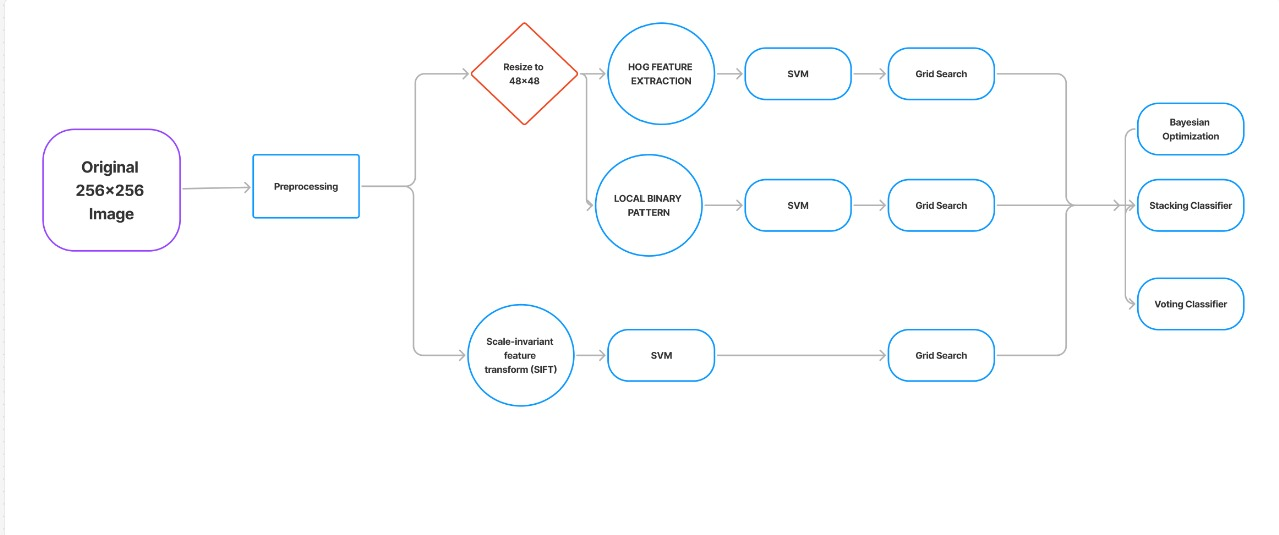
\includegraphics[width=\linewidth]{1.png}
    \caption{Work Flowchart}
\end{figure}

Our mid-semester project explored various feature extraction techniques, including LBP, SIFT, and HOG, to classify images. In this phase, we aim to combine these features by performing hyperparameter tuning(on a smaller sample than the dataset) using grid search and applying ensemble learning methods to enhance classification performance. This approach leverages the strengths of multiple models for improved accuracy.\\
The following hyperparameters were identified as the best according to the grid search algorithm:

\begin{itemize}[noitemsep, topsep=0pt]
    \item \textbf{SIFT}
    \begin{itemize}[noitemsep, topsep=0pt]
        \item Best Accuracy: 61.00\%
        \item Best SIFT Parameters: \texttt{n\_features=256, contrast\_threshold=0.06, edge\_threshold=5}
        \item Best SVM Parameters: \{\texttt{'C': 0.1, 'kernel': 'linear'}\}
    \end{itemize}

    \item \textbf{HOG}
    \begin{itemize}[noitemsep, topsep=0pt]
        \item Best HOG Parameters: \{\texttt{'pixels\_per\_cell': (8, 8), 'cells\_per\_block': (3, 3), 'orientations': 9}\}
        \item Validation Accuracy: 0.6892857142857143
    \end{itemize}

    \item \textbf{LBP}
    \begin{itemize}[noitemsep, topsep=0pt]
        \item Best LBP Parameters: \{\texttt{'radius': 2, 'n\_points': 8, 'method': 'uniform'}\}
        \item Validation Accuracy: 0.6000
    \end{itemize}
\end{itemize}

We applied ensemble learning to combine models trained on HOG, LBP, and SIFT features. The Voting Classifier uses majority voting, ensuring stability and leveraging the strengths of individual models. The Stacking Classifier uses a meta-classifier to combine predictions optimally, capturing inter-model relationships. These methods enhance classification accuracy and robustness by integrating diverse feature representations.

\subsection{Convolutional Neural Networks (CNNs)}

\subsubsection{Preprocessing}
We normalized the image input by dividing the pixel by 255; this converts the image pixel to a range of [0, 1]. This step is crucial as it could accelerate the convergence process. Additionally, we also resized the image to 128x128 to ensure uniformity.

\subsubsection{Grid Search}
We used a custom grid search to optimize our hyperparameters; some of the optimizers we used are \texttt{Adam} and \texttt{RMSprop}. We compared two learning rates (\(0.001\) and \(0.0001\)) and batch sizes (\(32\) and \(64\)). Each combination was evaluated to identify the optimal parameters that gave the best accuracy and minimum loss on the validation dataset. We applied the grid search on a smaller dataset as it would have consumed much time. This approach helped us to fine-tune our model and get optimal performance. Out of them, the best model was the \{\texttt{'batch\_size': 32, 'learning\_rate': 0.001, 'optimizer': 'rmsprop'}\}.

\begin{figure}[H]
    \centering
    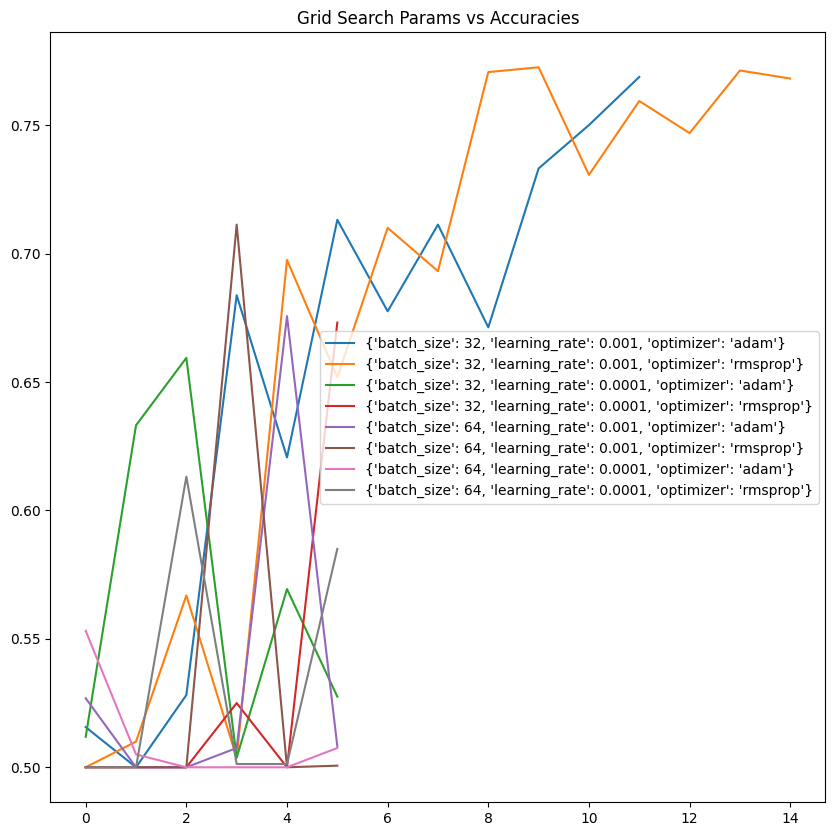
\includegraphics[scale=0.3]{7.png}
    \caption{Work Flowchart}
\end{figure}

\subsubsection{Methodology}
The literature review conducted by us showed that one of the most promising ways to detect deepfake images has been through the use of Convolutional Neural Networks (CNNs). The inbuilt ability to learn spatial hierarchies and features makes it ideal for this task. 
\\\\
The CNN architecture we used consists of four convolutional layers (with increasing filter sizes of 32, 64, 64, and 128), each followed by batch normalization, max pooling, and dropout with 0.2 probability. The model ends with a dense layer of 256 neurons, and we have used a SoftMax output layer for binary classification. The use of dropout and batch normalization helps speed up the training, regularize, and prevent overfitting. The increasing number of filters in the convolutional layers helps capture progressively more complex features as the layers go deeper. A large dense layer of 256 neurons was used, allowing the model to learn more complex patterns.
\\\\
We trained the model for 20 epochs with early stopping to prevent overfitting and capture the best performance on the validation set. The early stopping mechanism monitored the validation loss, with a patience of 6 epochs, triggering when the loss did not improve by more than 0.001.

\section{Results and Analysis}

\subsection{Classical Machine Learning}

\textbf{Voting Classifier Test Accuracy: 0.72}

\textbf{Stacking Classifier Accuracy: 0.78}
\\\\
The results demonstrate that the Stacking Classifier achieved higher accuracy (78\%) than the Voting Classifier (72\%). This highlights the effectiveness of stacking in learning inter-model relationships and optimally combining predictions, as opposed to the more straightforward majority voting approach, thereby better utilizing the diverse feature sets.

\subsection{Convolutional Neural Networks (CNNs)}

\section*{Results}

The CNN model trained on the best hyperparameters obtained from the grid search resulted in the following validation vs. training accuracy and loss graphs:

\begin{figure}[H]
    \centering
    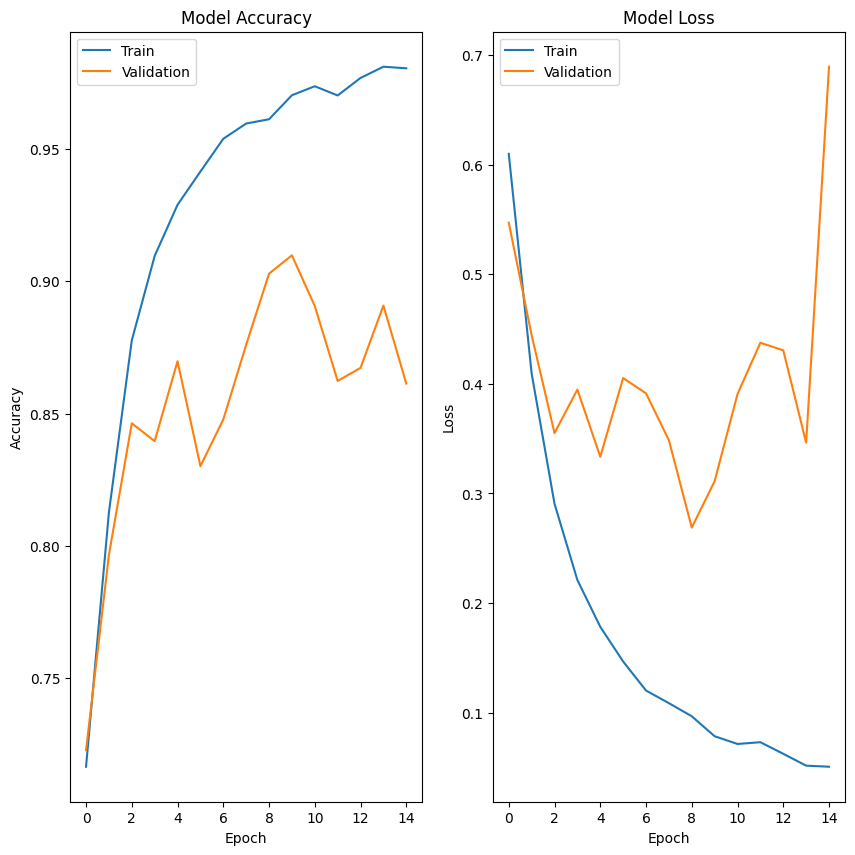
\includegraphics[scale=0.4]{8.png}
    \caption{Work Flowchart}
\end{figure}

The model achieved a validation accuracy of approximately 90.28\%, demonstrating its effectiveness in distinguishing between real and deepfake images. During training, the validation loss initially decreased, then fluctuated before stabilizing, prompting early stopping to prevent overfitting. 

The final model was evaluated on the test set, where it also achieved an accuracy of 84.764\%, confirming its strong generalization ability.


\section{Conclusion}

This work discussed the application of classical machine learning methods and CNN for image classification, in particular, detecting deepfakes. From this study, it was apparent that the different feature extraction techniques, HOG, LBP, SIFT combined with ensemble learning, do pretty well. Experimentally, it has been proved that the test accuracy by the Stacking Classifier at 78\% is significantly better than the Voting Classifier at 72\%. So, the inter-model relationship pays off to leverage it.
\\\\
CNNs significantly outperformed classical approaches, achieving a validation accuracy of 90.28\% and a test accuracy of 84.76\%. The use of grid search for hyperparameter optimization and architectural elements like dropout, batch normalization, and early stopping contributed to improved performance and generalization.
\\\\
Overall, the results emphasize the superiority of CNNs in deepfake detection task. We explored how well traditional could perform in such a field like image classification where models like CNNs dominate the field. We were able to achieve quite high accuracy results with the traditional models too displaying their capability in this field too.
\\\\
\subsection{contributions}
\begin{itemize}
    \item Himang Chandra Garg: Worked on the CNN model, data preprocessing, and hyperparameter tuning.
    \item Dasari Sai Harsh: Worked on the classical machine learning models, feature extraction, and ensemble learning.
    \item Nishil Agarwal: Worked on the dataset analysis, data visualization, and hyperparameter tuning.
    \item Piyush Narula: Worked on the dataset analysis, data visualization, and hyperparameter tuning.
\end{itemize}

\begin{thebibliography}{6}
    \bibitem{SIFT} Detecting Fake Images Using Machine Learning. Available: \url{https://ijrpr.com/uploads/V4ISSUE4/IJRPR11629.pdf}
    \bibitem{SIFT} Deep Learning for Image Authentication: A Comparative Study on Real and AI-Generated Image Classification. Available: \url{https://www.researchgate.net/publication/375952278_Deep_Learning_for_Image_Authentication_A_Comparative_Study_on_Real_and_AI-Generated_Image_Classification}
    \bibitem{SIFT} Exploring and Analyzing Image Data with Python. Available: \href{https://medium.com/@sehjadkhoja0/title-exploring-and-analyzing-image-data-with-python-79a7f72f4d2b}{link}
    \bibitem{SIFT} SIFT (Scale-Invariant Feature Transform). Available: \url{https://docs.opencv.org/4.x/da/df5/tutorial_py_sift_intro.html}
    \bibitem{HOG} HOG (Histogram of Oriented Gradients). Available: \url{https://machinelearningmastery.com/opencv_hog/}
    \bibitem{LBP} Local Binary Pattern (LBP). Available: \href{https://aihalapathirana.medium.com/understanding-the-local-binary-pattern-lbp-a-powerful-method-for-texture-analysis-in-computer-4fb55b3ed8b8}{link}
    \bibitem{SVM} SVM (Support Vector Machine). Available: \url{https://scikit-learn.org/1.5/modules/svm.html}
    \bibitem{CNN} Keras-cnn-tutorial. Available: \url{https://victorzhou.com/blog/keras-cnn-tutorial}
    \bibitem{CNN} Image-classification-using-convolutional-neural-networks. Available: \url{https://www.analyticsvidhya.com/blog/2021/01/image-classification-using-convolutional-neural-networks-a-step-by-step-guide/}
    \bibitem{CNN} Building-and-using-a-convolutional-neural-network. Available: \url{https://rohan09.medium.com/building-and-using-a-convolutional-neural-network-cnn-for-image-classification-with-keras-and-7abf571f0abb}
\end{thebibliography}
    

\end{document}
